%---------------------------------------------------------------------------------------------------
% Tests
%---------------------------------------------------------------------------------------------------
\newpage
%\part{Anfang}
\chapter{Tests}\label{cap:Tests}

% Test driven development

When lots of puzzle pieces comes together it is sometimes difficult to see the big picture. The same happens during the software development process. Providing a bugfree application is a big task. Getting close to this goal testing is very important though. Different aspects of testing have to be taken into consideration. Unit, integration, and usability tests are common, but the testing devices are also worth mentioning. However, how profoundly one tests, that does not mean there is no bug anymore.

\section{Test devices}
Android Studio provides an integrated emulator tool. One can simulate popular mobile devices, like Nexus, Google Pixel, and others (see \ref{fig:testdevice_overview}).

\begin{figure}[H]
	\centering 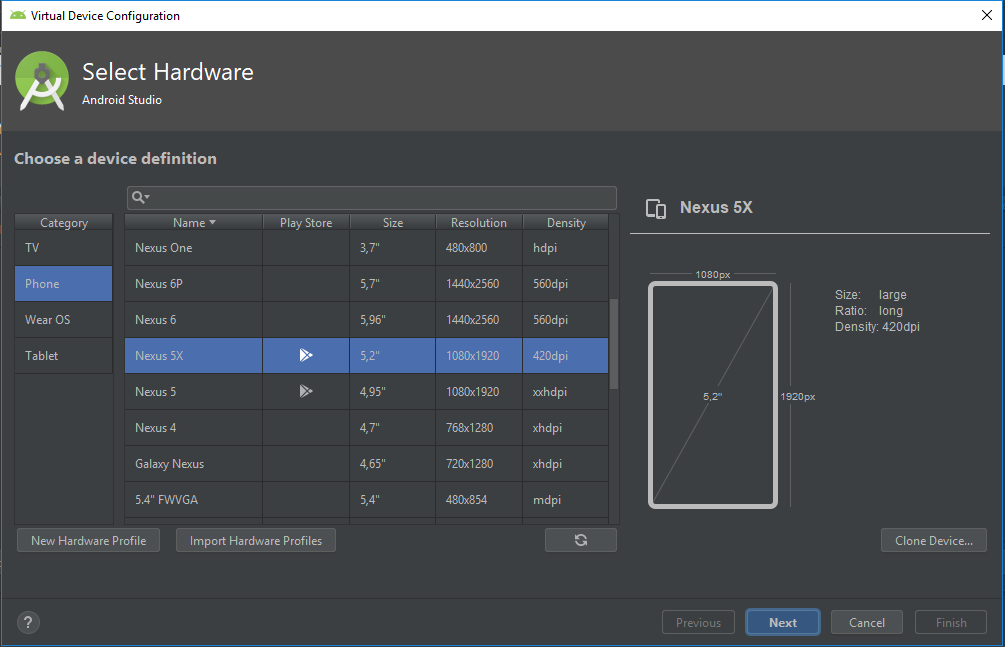
\includegraphics[width=0.8\textwidth]{test/testdevice_overview.PNG}
	\caption[Android Studio emulator overview]{Android Studio emulator overview}
	\label{fig:testdevice_overview}
\end{figure}

Or one can setup a custom device to fit their personal demands. There are plenty of tutorials with the topic "how to setup a custom emulator", so an exlaination will be out of scope of this thesis. 
Even though the Android Studio emulator is well done, emulator tests can not replace real device testing.
User expierience goes hand in hand with the haptical behaviour of the app. Therefore the Civitas app was also extensively tested on the developer devices, an \textit{UMIDIGI Z} and a \textit{Huawei P Smart (2019)}. 

An approach to make device testing more pleasant is realized with the VYZOR software. VYZOR acts like a mirrow and displays the device on to the computer monitor.  


\section{JUnit}
\begin{itemize}
\item test ApplicationClass.mArtefactList
\item test CategoryList 
\end{itemize}

\section{Integration Test}
man muss auf asyncCallback warten
bei erfolgreichem login


buttons work well
ich Teste